\PassOptionsToPackage{unicode=true}{hyperref} % options for packages loaded elsewhere
\PassOptionsToPackage{hyphens}{url}
%
\documentclass[]{article}
\usepackage{lmodern}
\usepackage{amssymb,amsmath}
\usepackage{ifxetex,ifluatex}
\usepackage{fixltx2e} % provides \textsubscript
\ifnum 0\ifxetex 1\fi\ifluatex 1\fi=0 % if pdftex
  \usepackage[T1]{fontenc}
  \usepackage[utf8]{inputenc}
  \usepackage{textcomp} % provides euro and other symbols
\else % if luatex or xelatex
  \usepackage{unicode-math}
  \defaultfontfeatures{Ligatures=TeX,Scale=MatchLowercase}
\fi
% use upquote if available, for straight quotes in verbatim environments
\IfFileExists{upquote.sty}{\usepackage{upquote}}{}
% use microtype if available
\IfFileExists{microtype.sty}{%
\usepackage[]{microtype}
\UseMicrotypeSet[protrusion]{basicmath} % disable protrusion for tt fonts
}{}
\IfFileExists{parskip.sty}{%
\usepackage{parskip}
}{% else
\setlength{\parindent}{0pt}
\setlength{\parskip}{6pt plus 2pt minus 1pt}
}
\usepackage{hyperref}
\hypersetup{
            pdftitle={Urine\_Creatinine\_Perchlorate},
            pdfauthor={Jenna Honan},
            pdfborder={0 0 0},
            breaklinks=true}
\urlstyle{same}  % don't use monospace font for urls
\usepackage[margin=1in]{geometry}
\usepackage{color}
\usepackage{fancyvrb}
\newcommand{\VerbBar}{|}
\newcommand{\VERB}{\Verb[commandchars=\\\{\}]}
\DefineVerbatimEnvironment{Highlighting}{Verbatim}{commandchars=\\\{\}}
% Add ',fontsize=\small' for more characters per line
\usepackage{framed}
\definecolor{shadecolor}{RGB}{248,248,248}
\newenvironment{Shaded}{\begin{snugshade}}{\end{snugshade}}
\newcommand{\AlertTok}[1]{\textcolor[rgb]{0.94,0.16,0.16}{#1}}
\newcommand{\AnnotationTok}[1]{\textcolor[rgb]{0.56,0.35,0.01}{\textbf{\textit{#1}}}}
\newcommand{\AttributeTok}[1]{\textcolor[rgb]{0.77,0.63,0.00}{#1}}
\newcommand{\BaseNTok}[1]{\textcolor[rgb]{0.00,0.00,0.81}{#1}}
\newcommand{\BuiltInTok}[1]{#1}
\newcommand{\CharTok}[1]{\textcolor[rgb]{0.31,0.60,0.02}{#1}}
\newcommand{\CommentTok}[1]{\textcolor[rgb]{0.56,0.35,0.01}{\textit{#1}}}
\newcommand{\CommentVarTok}[1]{\textcolor[rgb]{0.56,0.35,0.01}{\textbf{\textit{#1}}}}
\newcommand{\ConstantTok}[1]{\textcolor[rgb]{0.00,0.00,0.00}{#1}}
\newcommand{\ControlFlowTok}[1]{\textcolor[rgb]{0.13,0.29,0.53}{\textbf{#1}}}
\newcommand{\DataTypeTok}[1]{\textcolor[rgb]{0.13,0.29,0.53}{#1}}
\newcommand{\DecValTok}[1]{\textcolor[rgb]{0.00,0.00,0.81}{#1}}
\newcommand{\DocumentationTok}[1]{\textcolor[rgb]{0.56,0.35,0.01}{\textbf{\textit{#1}}}}
\newcommand{\ErrorTok}[1]{\textcolor[rgb]{0.64,0.00,0.00}{\textbf{#1}}}
\newcommand{\ExtensionTok}[1]{#1}
\newcommand{\FloatTok}[1]{\textcolor[rgb]{0.00,0.00,0.81}{#1}}
\newcommand{\FunctionTok}[1]{\textcolor[rgb]{0.00,0.00,0.00}{#1}}
\newcommand{\ImportTok}[1]{#1}
\newcommand{\InformationTok}[1]{\textcolor[rgb]{0.56,0.35,0.01}{\textbf{\textit{#1}}}}
\newcommand{\KeywordTok}[1]{\textcolor[rgb]{0.13,0.29,0.53}{\textbf{#1}}}
\newcommand{\NormalTok}[1]{#1}
\newcommand{\OperatorTok}[1]{\textcolor[rgb]{0.81,0.36,0.00}{\textbf{#1}}}
\newcommand{\OtherTok}[1]{\textcolor[rgb]{0.56,0.35,0.01}{#1}}
\newcommand{\PreprocessorTok}[1]{\textcolor[rgb]{0.56,0.35,0.01}{\textit{#1}}}
\newcommand{\RegionMarkerTok}[1]{#1}
\newcommand{\SpecialCharTok}[1]{\textcolor[rgb]{0.00,0.00,0.00}{#1}}
\newcommand{\SpecialStringTok}[1]{\textcolor[rgb]{0.31,0.60,0.02}{#1}}
\newcommand{\StringTok}[1]{\textcolor[rgb]{0.31,0.60,0.02}{#1}}
\newcommand{\VariableTok}[1]{\textcolor[rgb]{0.00,0.00,0.00}{#1}}
\newcommand{\VerbatimStringTok}[1]{\textcolor[rgb]{0.31,0.60,0.02}{#1}}
\newcommand{\WarningTok}[1]{\textcolor[rgb]{0.56,0.35,0.01}{\textbf{\textit{#1}}}}
\usepackage{graphicx,grffile}
\makeatletter
\def\maxwidth{\ifdim\Gin@nat@width>\linewidth\linewidth\else\Gin@nat@width\fi}
\def\maxheight{\ifdim\Gin@nat@height>\textheight\textheight\else\Gin@nat@height\fi}
\makeatother
% Scale images if necessary, so that they will not overflow the page
% margins by default, and it is still possible to overwrite the defaults
% using explicit options in \includegraphics[width, height, ...]{}
\setkeys{Gin}{width=\maxwidth,height=\maxheight,keepaspectratio}
\setlength{\emergencystretch}{3em}  % prevent overfull lines
\providecommand{\tightlist}{%
  \setlength{\itemsep}{0pt}\setlength{\parskip}{0pt}}
\setcounter{secnumdepth}{0}
% Redefines (sub)paragraphs to behave more like sections
\ifx\paragraph\undefined\else
\let\oldparagraph\paragraph
\renewcommand{\paragraph}[1]{\oldparagraph{#1}\mbox{}}
\fi
\ifx\subparagraph\undefined\else
\let\oldsubparagraph\subparagraph
\renewcommand{\subparagraph}[1]{\oldsubparagraph{#1}\mbox{}}
\fi

% set default figure placement to htbp
\makeatletter
\def\fps@figure{htbp}
\makeatother


\title{Urine\_Creatinine\_Perchlorate}
\author{Jenna Honan}
\date{9/5/2022}

\begin{document}
\maketitle

\hypertarget{merging-datasets-for-analysis}{%
\subsection{Merging Datasets for
Analysis}\label{merging-datasets-for-analysis}}

\begin{Shaded}
\begin{Highlighting}[]
\KeywordTok{unique}\NormalTok{(Creatinine}\OperatorTok{$}\NormalTok{Units)}
\end{Highlighting}
\end{Shaded}

\begin{verbatim}
## [1] "mg/dL"
\end{verbatim}

\begin{Shaded}
\begin{Highlighting}[]
\KeywordTok{unique}\NormalTok{(Perchlorate}\OperatorTok{$}\NormalTok{Units)}
\end{Highlighting}
\end{Shaded}

\begin{verbatim}
## [1] "ng/mL"
\end{verbatim}

\begin{Shaded}
\begin{Highlighting}[]
\NormalTok{Urine_Perch_Creat <-}\StringTok{ }\KeywordTok{merge}\NormalTok{(Creatinine, Perchlorate, }\DataTypeTok{by=}\KeywordTok{c}\NormalTok{(}\StringTok{"Sample ID"}\NormalTok{), }\DataTypeTok{all =}\NormalTok{ T)}
\NormalTok{Urine_Perch_Creat <-}\StringTok{ }\KeywordTok{as.data.frame}\NormalTok{(Urine_Perch_Creat)}
\NormalTok{Urine_Perch_Creat <-}\StringTok{ }\NormalTok{Urine_Perch_Creat[, }\KeywordTok{c}\NormalTok{(}\StringTok{"Sample ID"}\NormalTok{, }\StringTok{"Result.x"}\NormalTok{, }\StringTok{"LOD.x"}\NormalTok{, }\StringTok{"Result.y"}\NormalTok{, }\StringTok{"LOD.y"}\NormalTok{)]}
\KeywordTok{colnames}\NormalTok{(Urine_Perch_Creat) <-}\StringTok{ }\KeywordTok{c}\NormalTok{(}\StringTok{"Sample_ID"}\NormalTok{, }\StringTok{"Result_C_mg_dL"}\NormalTok{, }\StringTok{"LOD_C"}\NormalTok{, }\StringTok{"Result_P_ng_mL"}\NormalTok{, }\StringTok{"LOD_P"}\NormalTok{)}

\NormalTok{Urine_Perch_Creat}\OperatorTok{$}\NormalTok{Result_C[Urine_Perch_Creat}\OperatorTok{$}\NormalTok{Result_C}\OperatorTok{==}\StringTok{"NR"}\NormalTok{] <-}\StringTok{ }\OtherTok{NA}

\CommentTok{#Of the 297 observations, 2 have missing values for both creatinine and perchlorate, and 1 has missing value for creatinine but measured values for perchlorate, such that 294 obersvations are paired with measured values.}

\KeywordTok{library}\NormalTok{(dplyr)}
\end{Highlighting}
\end{Shaded}

\begin{verbatim}
## 
## Attaching package: 'dplyr'
\end{verbatim}

\begin{verbatim}
## The following objects are masked from 'package:stats':
## 
##     filter, lag
\end{verbatim}

\begin{verbatim}
## The following objects are masked from 'package:base':
## 
##     intersect, setdiff, setequal, union
\end{verbatim}

\begin{Shaded}
\begin{Highlighting}[]
\NormalTok{Urine_Perch_Creat }\OperatorTok\StringTok{ }
\StringTok{  }\KeywordTok{filter}\NormalTok{(}\OperatorTok{!}\KeywordTok{is.na}\NormalTok{(Result_C_mg_dL)) }\OperatorTok\StringTok{ }
\StringTok{  }\KeywordTok{summarise}\NormalTok{(}\StringTok{"n Creatinine < LOD"}\NormalTok{=}\KeywordTok{sum}\NormalTok{(Result_C_mg_dL}\OperatorTok{<}\NormalTok{LOD_C),}
            \StringTok{"n Perchlorate < LOD"}\NormalTok{=}\KeywordTok{sum}\NormalTok{(Result_P_ng_mL}\OperatorTok{<}\NormalTok{LOD_P))}
\end{Highlighting}
\end{Shaded}

\begin{verbatim}
##   n Creatinine < LOD n Perchlorate < LOD
## 1                  0                  NA
\end{verbatim}

\begin{Shaded}
\begin{Highlighting}[]
\CommentTok{#Rows with missing data for either creatinine or perchorate have been removed from the dataset (DF=99%). No replacement needed - all detected values above LOD.}
\end{Highlighting}
\end{Shaded}

\hypertarget{checking-distributions}{%
\subsection{Checking Distributions}\label{checking-distributions}}

\begin{Shaded}
\begin{Highlighting}[]
\KeywordTok{hist}\NormalTok{(}\KeywordTok{as.numeric}\NormalTok{(Urine_Perch_Creat}\OperatorTok{$}\NormalTok{Result_C_mg_dL), }\DataTypeTok{xlab =} \StringTok{"Creatinine (mg/dL)"}\NormalTok{)}
\end{Highlighting}
\end{Shaded}

\begin{verbatim}
## Warning in hist(as.numeric(Urine_Perch_Creat$Result_C_mg_dL), xlab = "Creatinine
## (mg/dL)"): NAs introduced by coercion
\end{verbatim}

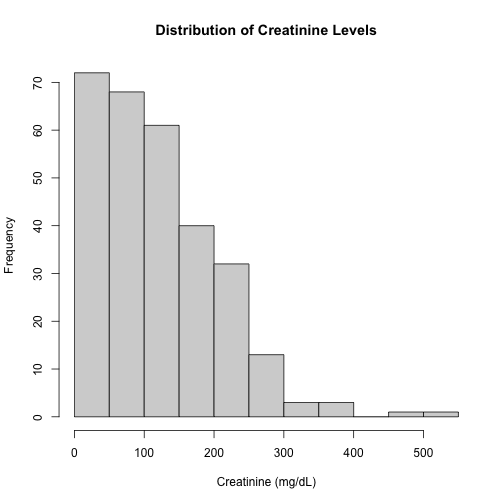
\includegraphics{Urine_Creatinine_Perchlorate_files/figure-latex/distributions-1.pdf}

\begin{Shaded}
\begin{Highlighting}[]
\KeywordTok{hist}\NormalTok{(}\KeywordTok{as.numeric}\NormalTok{(Urine_Perch_Creat}\OperatorTok{$}\NormalTok{Result_P_ng_mL), }\DataTypeTok{xlab =} \StringTok{"Perchlorate (ng/mL)"}\NormalTok{)}
\end{Highlighting}
\end{Shaded}

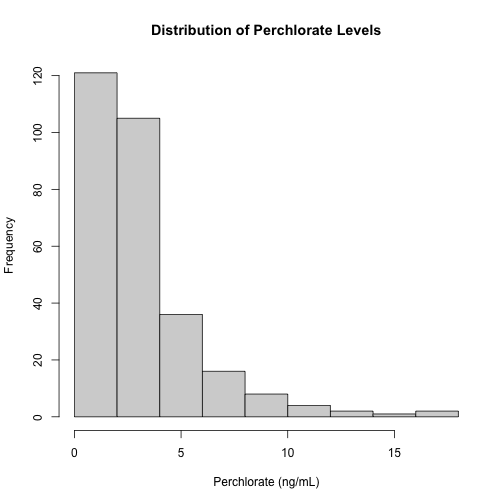
\includegraphics{Urine_Creatinine_Perchlorate_files/figure-latex/distributions-2.pdf}

\begin{Shaded}
\begin{Highlighting}[]
\KeywordTok{hist}\NormalTok{(}\KeywordTok{log}\NormalTok{(}\KeywordTok{as.numeric}\NormalTok{(Urine_Perch_Creat}\OperatorTok{$}\NormalTok{Result_C_mg_dL)), }\DataTypeTok{xlab =} \StringTok{"ln Creatinine (mg/dL)"}\NormalTok{)}
\end{Highlighting}
\end{Shaded}

\begin{verbatim}
## Warning in hist(log(as.numeric(Urine_Perch_Creat$Result_C_mg_dL)), xlab = "ln
## Creatinine (mg/dL)"): NAs introduced by coercion
\end{verbatim}

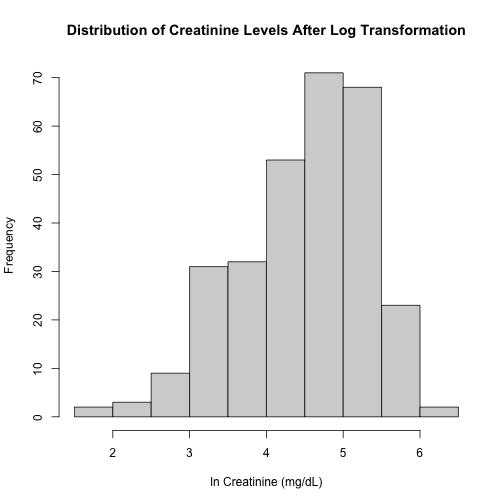
\includegraphics{Urine_Creatinine_Perchlorate_files/figure-latex/distributions-3.pdf}

\begin{Shaded}
\begin{Highlighting}[]
\KeywordTok{hist}\NormalTok{(}\KeywordTok{log}\NormalTok{(}\KeywordTok{as.numeric}\NormalTok{(Urine_Perch_Creat}\OperatorTok{$}\NormalTok{Result_P_ng_mL)), }\DataTypeTok{xlab =} \StringTok{"ln Perchlorate (ng/mL)"}\NormalTok{)}
\end{Highlighting}
\end{Shaded}

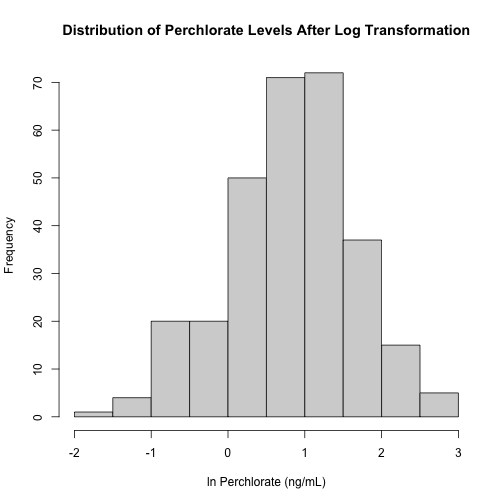
\includegraphics{Urine_Creatinine_Perchlorate_files/figure-latex/distributions-4.pdf}

\hypertarget{analyzing-correlation-of-creatinine-and-perchlorate}{%
\subsection{Analyzing Correlation of Creatinine and
Perchlorate}\label{analyzing-correlation-of-creatinine-and-perchlorate}}

\begin{Shaded}
\begin{Highlighting}[]
\KeywordTok{library}\NormalTok{(ggplot2)}

\KeywordTok{ggplot}\NormalTok{(Urine_Perch_Creat, }\KeywordTok{aes}\NormalTok{(}\DataTypeTok{x=}\KeywordTok{as.numeric}\NormalTok{(Result_C_mg_dL), }\DataTypeTok{y=}\KeywordTok{as.numeric}\NormalTok{(Result_P_ng_mL)))}\OperatorTok{+}
\StringTok{  }\KeywordTok{geom_point}\NormalTok{()}\OperatorTok{+}
\StringTok{  }\KeywordTok{geom_smooth}\NormalTok{(}\DataTypeTok{method=}\NormalTok{lm, }\DataTypeTok{se=}\NormalTok{F)}\OperatorTok{+}
\StringTok{  }\KeywordTok{xlab}\NormalTok{(}\StringTok{"Creatinine (mg/dL)"}\NormalTok{)}\OperatorTok{+}
\StringTok{  }\KeywordTok{ylab}\NormalTok{(}\StringTok{"Perchlorate (ng/mL)"}\NormalTok{)}\OperatorTok{+}
\StringTok{  }\KeywordTok{ggtitle}\NormalTok{(}\StringTok{"Correlation of Perchlorate and Creatinine"}\NormalTok{)}
\end{Highlighting}
\end{Shaded}

\begin{verbatim}
## Warning in FUN(X[[i]], ...): NAs introduced by coercion

## Warning in FUN(X[[i]], ...): NAs introduced by coercion

## Warning in FUN(X[[i]], ...): NAs introduced by coercion
\end{verbatim}

\begin{verbatim}
## `geom_smooth()` using formula 'y ~ x'
\end{verbatim}

\begin{verbatim}
## Warning: Removed 3 rows containing non-finite values (stat_smooth).
\end{verbatim}

\begin{verbatim}
## Warning: Removed 3 rows containing missing values (geom_point).
\end{verbatim}

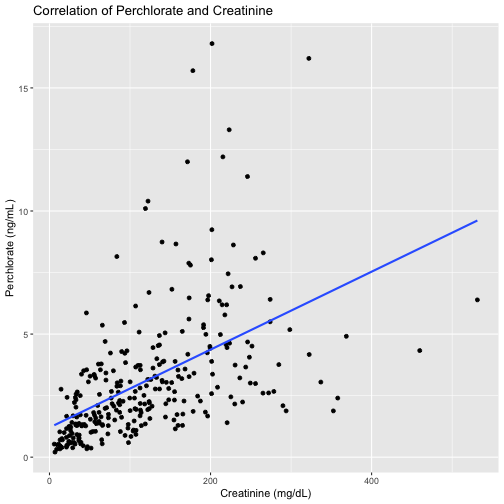
\includegraphics{Urine_Creatinine_Perchlorate_files/figure-latex/correlation-1.pdf}

\begin{Shaded}
\begin{Highlighting}[]
\KeywordTok{ggplot}\NormalTok{(Urine_Perch_Creat, }\KeywordTok{aes}\NormalTok{(}\DataTypeTok{x=}\KeywordTok{log}\NormalTok{(}\KeywordTok{as.numeric}\NormalTok{(Result_C_mg_dL)), }\DataTypeTok{y=}\KeywordTok{log}\NormalTok{(}\KeywordTok{as.numeric}\NormalTok{(Result_P_ng_mL))))}\OperatorTok{+}
\StringTok{  }\KeywordTok{geom_point}\NormalTok{()}\OperatorTok{+}
\StringTok{  }\KeywordTok{geom_smooth}\NormalTok{(}\DataTypeTok{method=}\NormalTok{lm, }\DataTypeTok{se=}\NormalTok{F)}\OperatorTok{+}
\StringTok{  }\KeywordTok{xlab}\NormalTok{(}\StringTok{"ln Creatinine (mg/dL)"}\NormalTok{)}\OperatorTok{+}
\StringTok{  }\KeywordTok{ylab}\NormalTok{(}\StringTok{"ln Perchlorate (ng/mL)"}\NormalTok{)}\OperatorTok{+}
\StringTok{  }\KeywordTok{ggtitle}\NormalTok{(}\StringTok{"Correlation of Perchlorate and Creatinine After Log Transformation"}\NormalTok{)}
\end{Highlighting}
\end{Shaded}

\begin{verbatim}
## Warning in FUN(X[[i]], ...): NAs introduced by coercion
\end{verbatim}

\begin{verbatim}
## Warning in FUN(X[[i]], ...): NAs introduced by coercion

## Warning in FUN(X[[i]], ...): NAs introduced by coercion
\end{verbatim}

\begin{verbatim}
## `geom_smooth()` using formula 'y ~ x'
\end{verbatim}

\begin{verbatim}
## Warning: Removed 3 rows containing non-finite values (stat_smooth).
\end{verbatim}

\begin{verbatim}
## Warning: Removed 3 rows containing missing values (geom_point).
\end{verbatim}

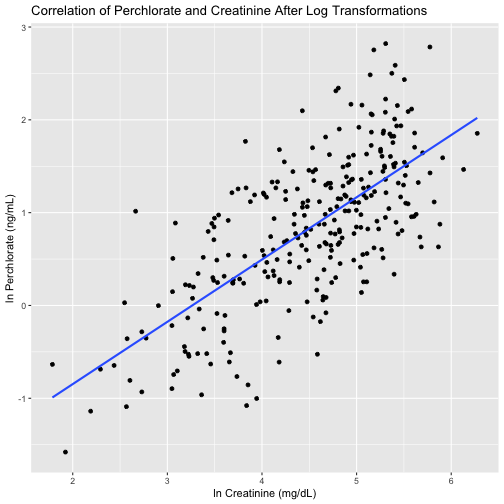
\includegraphics{Urine_Creatinine_Perchlorate_files/figure-latex/correlation-2.pdf}

\begin{Shaded}
\begin{Highlighting}[]
\KeywordTok{cor.test}\NormalTok{(}\KeywordTok{log}\NormalTok{(}\KeywordTok{as.numeric}\NormalTok{(Urine_Perch_Creat}\OperatorTok{$}\NormalTok{Result_C_mg_dL)), }\KeywordTok{log}\NormalTok{(}\KeywordTok{as.numeric}\NormalTok{(Urine_Perch_Creat}\OperatorTok{$}\NormalTok{Result_P_ng_mL)))}
\end{Highlighting}
\end{Shaded}

\begin{verbatim}
## Warning in cor.test(log(as.numeric(Urine_Perch_Creat$Result_C_mg_dL)),
## log(as.numeric(Urine_Perch_Creat$Result_P_ng_mL))): NAs introduced by coercion
\end{verbatim}

\begin{verbatim}
## 
##  Pearson's product-moment correlation
## 
## data:  log(as.numeric(Urine_Perch_Creat$Result_C_mg_dL)) and log(as.numeric(Urine_Perch_Creat$Result_P_ng_mL))
## t = 16.696, df = 292, p-value < 2.2e-16
## alternative hypothesis: true correlation is not equal to 0
## 95 percent confidence interval:
##  0.6352580 0.7530543
## sample estimates:
##       cor 
## 0.6988647
\end{verbatim}

\end{document}
